\documentclass[class=scrartcl, crop=false]{standalone}
\usepackage[
typ={ohne},
fach=Informatik,
lerngruppe=SG-J1,
%loesungen=seite,
%lizenz={cc-by-nc-sa-4}
module={Aufgaben},
farbig
]{schule}
%\usepackage{polyglossia}
%\setmainlanguage{ngerman}
\usepackage[subpreambles=true]{standalone}
\usepackage{import}
\usepackage{fourier-otf}
\setmonofont{Ubuntu Mono Regular}[Scale=0.9]
\usepackage{shellesc}
\ShellEscape{pythontex \jobname.pytxcode }
\usepackage[
%prettyprinter=pygments, %pygopt={style=emacs}
]{pythontex}


\usepackage{hyperref}


\usepackage{booktabs}

\usepackage{minted}





\newcommand{\expandpyconc}[1]{\expandafter\reallyexpandpyconc\expandafter{#1}}
\newcommand{\reallyexpandpyconc}[1]{\pyconc{exec(compile(open('#1', 'rb').read(), '#1', 'exec'))}}

\newenvironment{pyconcodeblck}[1]
{\newcommand{\snippetfile}{snippet-#1.py}
	\VerbatimEnvironment
	\begin{VerbatimOut}{\snippetfile}}
	{\end{VerbatimOut}
	\expandpyconc{\snippetfile}}

\newcommand{\typesetcode}[1]{\inputpygments{python}{snippet-#1.py}}



\begin{document}

\begin{pyconcodeblck}{while_schleifen}
def power_of_two(x):
    i = 1
    while i < x:
        i = i * 2    
    return i == x


def halving_sum(n): 
    acc = 0
    while n >= 1:
        acc = acc + n
        n = n//2
    return acc




def nb_year(p0, percent, aug, p):
    percent =  1 + percent/100
    years = 0
    while p0 < p:
        p0 = int(p0* percent) + aug
        years = years + 1
    return years


def is_square(n):    
    i = 0
    while i * i < n:
        i = i + 1
    return i * i == n

def next_collatz(n):
    if n % 2 == 0:
        return n // 2
    else:
        return 3 * n + 1


def hotpo(n):
    counter = 0
    while n != 1:
        n = next_collatz(n)
        counter = counter + 1
    return counter



def collatz(n):
    acc = str(n)
    while n != 1:
        n = next_collatz(n)
        acc = acc + "->" + str(n)
    return acc


\end{pyconcodeblck}

\section{While-Schleifen}

\begin{aufgabe} \noindent
Implementiere eine Funktion \mintinline{python}{guessing_game()}. Diese Funktion hat keine Parameter. Beim Aufruf fragt sie nach, welche Zahl erraten werden soll. Anschließend wird solange geraten bis diese Zahl eingegeben wurde.

\begin{figure}[H]
	%\centerline{\includesvg[inkscapelatex=false,width=0.5\linewidth]{rock-paper-scissors}}
	\centering	
	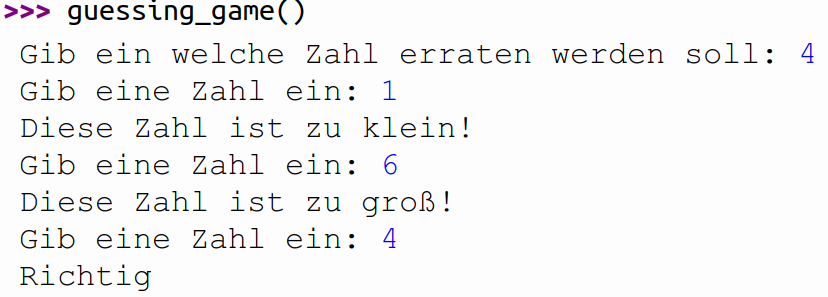
\includegraphics[width=0.7\linewidth]{guessing_game}

\end{figure}

\end{aufgabe}

\begin{aufgabe}
Erweitere die Funktion  \mintinline{python}{guessing_game()}, um einen Zähler für die Anzahl der benötigten Versuche. Beim Ende des Spiels soll ausgegeben werden, wie viele Versuche der Spieler benötigt hat.  
\end{aufgabe}

\begin{aufgabe} \noindent
Implementiere eine Funktion \mintinline{python}{power_of_two}, die prüft, ob eine nicht negative ganze Zahl eine Zweierpotenz ist. 

\begin{pyconsole}
power_of_two(0)
power_of_two(1)
power_of_two(2)
power_of_two(5)
power_of_two(16)
\end{pyconsole}

\noindent\url{https://www.codewars.com/kata/534d0a229345375d520006a0/train/python}

\end{aufgabe}



\begin{aufgabe} \noindent
Implementiere eine Funktion \mintinline{python}{halving_sum}, die für eine positive Zahl $n$ die Summe $$ \mathtt{n + n//2 + n//4 + \dots + 1 } $$ berechnet. Z.B. gilt $\mathtt{halving\_sum(25) = 25 + 12 + 6 + 3 + 1 = 47}$.

\begin{pyconsole}
halving_sum(25)
halving_sum(1)
\end{pyconsole}

\noindent\url{https://www.codewars.com/kata/5a58d46cfd56cb4e8600009d/train/python}

\end{aufgabe}


\begin{aufgabe} \noindent
Implementiere eine Funktion \mintinline{python}{nb_year}, die berechnet wann eine Population mit gegebenem Anfangsbestand, jährlichem prozentualen Wachstum und jährlicher Zuwanderung eine bestimmte Grenze überschreitet.

Z.B. könnte man eine Kleinstadt mit $1000$ Einwohnern, einem jährlichen Wachstum von $2$ Prozent und $50 $ Personen, die jedes Jahr in die Stadt ziehen betrachten und sich fragen wann $1200$ Personen in der Stadt wohnen.

\begin{align*}
\textnormal{1. Jahr } & 1000 + 1000 * 0.02 + 50 = 1070 \textnormal{ Einwohner } \\
\textnormal{2. Jahr } & 1070 + 1070 * 0.02 + 50 = 1141 \textnormal{ Einwohner } \\
\textnormal{3. Jahr } & 1141 + 1141 * 0.02 + 50 = 1213  \textnormal{ Einwohner }
\end{align*}
Die Grenze ist also nach $3$ Jahren erreicht.\\ \hinweis{Beachte, dass ab dem 2. Jahr abgerundet wurde, da die Einwohnerzahl eine ganze Zahl sein muss.}

\begin{pyconsole}
nb_year(1000, 2 , 50 , 1200)
\end{pyconsole}

\noindent\url{https://www.codewars.com/kata/563b662a59afc2b5120000c6/train/python}

\end{aufgabe}





\begin{aufgabe} \noindent
Implementiere eine Funktion \mintinline{python}{is_square}, die prüft, ob eine natürliche Zahl eine Quadratzahl ist.

\begin{pyconsole}
is_square(0)
is_square(1)
is_square(2)
\end{pyconsole}

\noindent\url{https://www.codewars.com/kata/54c27a33fb7da0db0100040e/train/python}

\end{aufgabe}



\begin{aufgabe} \noindent
Collatz-Folgen werden nach dem folgenden Prinzip gebildet. 
\begin{enumerate}
	\item Wähle eine beliebige natürliche Zahl $n$
	\item  
		\begin{itemize}
		\item Wenn $n$ gerade ist, wähle als nächstes Folgenglied $\frac{n}{2}$
		\item Wenn $n$ ungerade ist, wähle als nächstes Folgenglied $3*n + 1$
		\end{itemize} 
	\item Wiederhole Schritt 2 immer wieder bis die Zahl $1$ erreicht ist.

\end{enumerate}

Formaler ausgedrückt, wird die folgende Funktion auf ein Folgenglied angewendet um das nächste Folgenglied zu erhalten.

$$f(n) = \begin{cases} n/2 &\textnormal{falls n gerade ist } \\ 3n+1 & \textnormal{falls n ungerade ist } \end{cases}$$


Z.B. erhält man für die Startzahl $5$ die folgende Collatz-Folge: $5, 16, 8, 4, 2, 1$

Implementiere eine Funktion \mintinline{python}{hotpo}, die berechnet wie viele der oben erklärten Berechnungen durchgeführt werden müssen, um von einer eingegeben Startzahl auf die Zahl $1$ zu kommen

\begin{pyconsole}
hotpo(1)
hotpo(5)
\end{pyconsole}

\noindent\url{https://www.codewars.com/kata/577a6e90d48e51c55e000217/train/python}
\end{aufgabe}



\begin{aufgabe} \noindent
Implementiere eine Funktion  \mintinline{python}{collatz}. Diese gibt einen String zurück, der alle Zwischenergebnisse der Collatz-Folge anzeigt, bis $1$ erreicht wurde.

\begin{pyconsole}
collatz(1)
collatz(5)
\end{pyconsole}
\noindent\url{https://www.codewars.com/kata/5286b2e162056fd0cb000c20/python}
\end{aufgabe}


\end{document}
